\documentclass{article}
\usepackage{graphicx} %For importing images
\usepackage[labelfont=bf]{caption} %For making "Figure i:" label bold
\usepackage{enumerate}
\usepackage{hyperref}
\usepackage[pass]{geometry}

\newenvironment{myindentpar}[1]
 {\begin{list}{}
         {\setlength{\leftmargin}{#1}}
         \item[]
 }
 {\end{list}}

\begin{document}

  \renewcommand\footnotemark{}
  \title{How Artificial Intelligence Affects the Work Force}
  \author{Michael Giancola \thanks{This White Paper was written for WR 1011 at Worcester Polytechnic Institute}}
  \date{February 19, 2016}
  \maketitle

  \cleardoublepage

  \newgeometry{left=1.875in,right=1.875in,top=1in,bottom=1.5in}

  \section{Introduction}
    \paragraph{}
      ``Advanced Robotics'', or in other words, artificially intelligent machines (AI),
      was identified by the McKinsey Global Institute as one of seven emerging
      technologies they expect will have a one trillion dollar or greater impact on the economy.$_{[1]}$
      Given McKinsey's prediction, AI will significantly influence much of the
      world economy. However, the impact of these changes on employment, wages,
      and productivity remains to be seen.
      Much of the impact of AI will depend on how well executives
      prepare their companies for the changing circumstances.

    \paragraph{}
      In a \textit{NarrativeScience} study, over 90\% of respondents said that
      their company uses AI primarily for automation.$_{[2]}$ In general, intelligent
      machines are used for automating repetitive tasks.
      The present economic impact of AI is clear in the manufacturing
      industry. Employment of manufacturing workers costs around \$6
      trillion, representing 19\% of global employment costs.$_{[1]}$

    \paragraph{}
      With the advent of true AI, much more sophisticated work will be able to
      be automated by machines. A truly intelligent machine would be able to
      replace most knowledge workers. That is, people whose job it is to think.
      This includes academics, engineers, insurance underwriters, lawyers, teachers,
      and physicians.
      The projected economic impact to knowledge workers could be even greater than
      in the manufacturing industry. Approximately \$9 trillion is spent on employing
      knowledge workers, representing 27\% of global employment costs.$_{[1]}$
      Experts at McKinsey predict that autonomous tools will be able to do the
      work of 110 to 140 million full time employees by 2025.$_{[1]}$

    \paragraph{}
      As is usually the case with emerging technology, corporate executives have
      two options: resist, or adapt. In this scenario, it seems advantageous for
      those involved to adapt. True AI is inevitable, and any company that
      refuses to adapt to the changing circumstances will be unable to compete
      in their market. Furthermore, if effected companies determine how to best
      use these tools (which do the work of 110 million people) in unison
      with the employees they have now, their productivity will increase exponentially.

  \section{Characteristics of Intelligence}

    \paragraph{}
      Current applications of AI can be seen in airport kiosks, Siri, and Google's
      autonomous car. Yet, it is difficult to define exactly what artificial
      intelligence is. AI can be categorized into three distinct groups: Dumb
      intelligence, simulated intelligence, and true intelligence.\\

    \begin{myindentpar}{1cm}
      Dumb Intelligence: These machines automate a simple task, usually by requesting
      data from a user and performing a task based on that data; hence, the
      oxymoronic name ``dumb'' intelligence. A simple example of this type of AI
      is an airport kiosk used to check in before a flight. They are not intelligent at all,
      they just follow a simple computer program. However, they are well known
      and relevant to the discussion of AI.\\

      Simulated Intelligence: These machines analyze the data that they
      receive in a way that makes them appear intelligent.
      For example, a GPS can find a route between two points, and even figure out what
      to do if there's a detour along the path. However, in reality it is just a
      simple algorithm processing a relatively small amount of data.\\

      True Intelligence: The machine should be able to perform some action,
      assess the consequences of its action, and, ultimately, learn from its
      successes and failures.
    \end{myindentpar}

    \paragraph{}
      Figure 1 shows results from a \textit{NarrativeScience} survey of 200 C-Suite
      executives about what they believe constitutes artificial intelligence.
      Respondents worked in a range of fields including technology, health care,
      and finance. Almost one third of people surveyed believe that
      artificial intelligence is a combination of the things listed in the graphic
      below.

    \paragraph{}
      The ability to learn and adapt is the hallmark of AI. However for AI to feel
      ``real'' to most people, it must be able to communicate in a
      reasonable manner. All of these components will come
      together in the next few decades as artificial intelligence continues to
      advance.

    \begin{figure}[ht]
      \centering
      \captionsetup{width=.85\linewidth}
      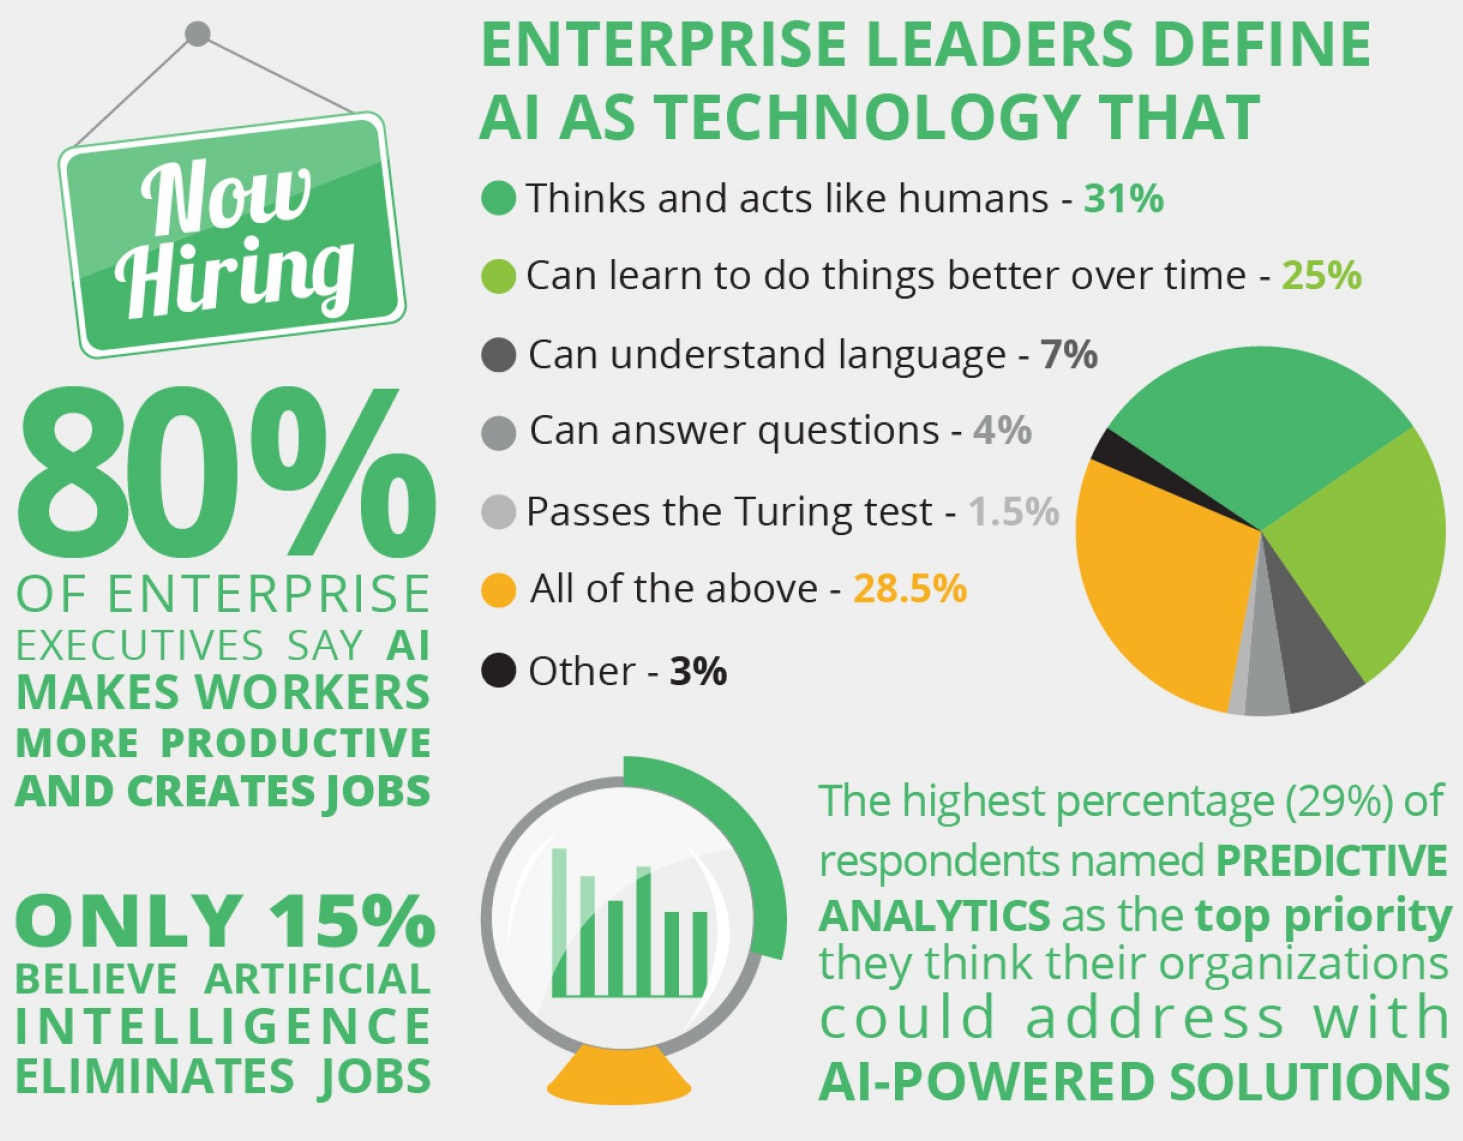
\includegraphics[width=0.85\textwidth,height=\textheight, keepaspectratio]{Figure1}
      \caption{Enterprise leaders are surveyed on their perceptions of AI in the workforce.
               \href{http://thumbnails-visually.netdna-ssl.com/artificial-intelligence-is-not-killing-jobs_557b4376e27b8_w1500.jpg}
               {\textbf{Source}}}
    \end{figure}

  \cleardoublepage

  \section{Current Effects}
    \paragraph{}
      According to \textit{NarrativeScience}, ``only 15\% [of people surveyed]
      believe that AI eliminates jobs''.$_{[2]}$ This statistic may initially
      appear counter to popular opinion. A Google search using the key words
      ``Artificial Intelligence Destroys Jobs'' produces more than a half million
      articles. However, this particular study from \textit{NarrativeScience}
      found that corporate leaders believe that AI may actually play a very
      positive role in the workplace. As the \textit{NarrativeScience} report
      wrote,

      \begin{center}
        \fbox{
          \parbox{0.75\textwidth}{
          ``...many executives are learning that AI-powered solutions can step in
          to solve the data-use and comprehension problem, provide a competitive
          advantage, free their employees to focus on strategic initiatives and even
          create jobs.''$_{[2]}$
          }
        }
      \end{center}

    \paragraph{}
      While this outlook is more positive, other studies still believe that AI has
      the potential to hurt the job market. Figure 2 compares
      the labor productivity in the US to the relative
      level of private employment. There is a strong correlation between both factors
      until the early 2000s, where the trend stops. Many economists, including
      Erik Brynjolfsson, believe this could be cause for concern.
      In an interview with TechRepublic, Brynjolfsson
      commented on this trend:

      \begin{center}
        \fbox{
          \parbox{0.75\textwidth}{
          ``Unlike much of the 20th century, we're now
          seeing a falling ratio of employment to population ...[we think] that
          many of the underlying trends in technology are likely to accelerate this
          so it’s something we need to pay some serious attention to.''$_{[3]}$
          }
        }
      \end{center}

      \begin{figure}[ht]
        \centering
        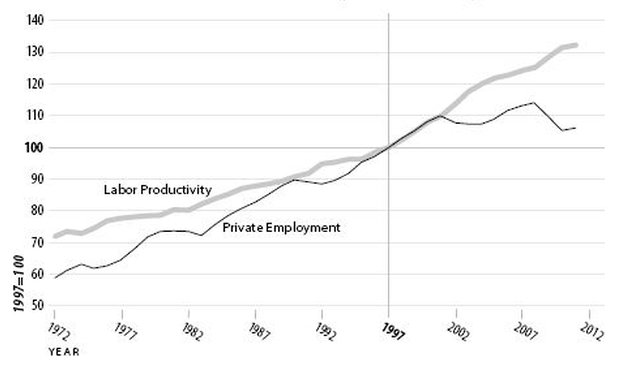
\includegraphics[width=\textwidth,height=\textheight, keepaspectratio]{Figure2}
        \caption{Labor Productivity vs. Private Employment.
                 \href{http://www.techrepublic.com/article/ai-is-destroying-more-jobs-than-it-creates-what-it-means-and-how-we-can-stop-it/}
                 {\textbf{Source}}}
      \end{figure}

    \paragraph{}
      Despite Brynjolfsson's concern, it is difficult to claim that AI was
      the sole cause for the disparity between labor productivity and private
      employment. Indeed, it is difficult to single out the effects of AI,
      especially because it is such a new development. The results of the
      \textit{NarrativeScience} study should be more closely considered.
      Even if, and in some cases, especially if, AI reduces employment and
      increases productivity, companies which utilize AI will have an advantage
      over their competitors who do not.

  \section{Collaboration of Man and Machine}

    \paragraph{}
      If companies are to improve their productivity by introducing intelligent
      machines to the workplace, how can these machines
       and humans best collaborate? More importantly, what will be the place
      of humans in the workforce, with robots doing a lot of the work that humans
      do now?

      \begin{figure}[ht]
        \centering
        \captionsetup{width=.85\linewidth}
        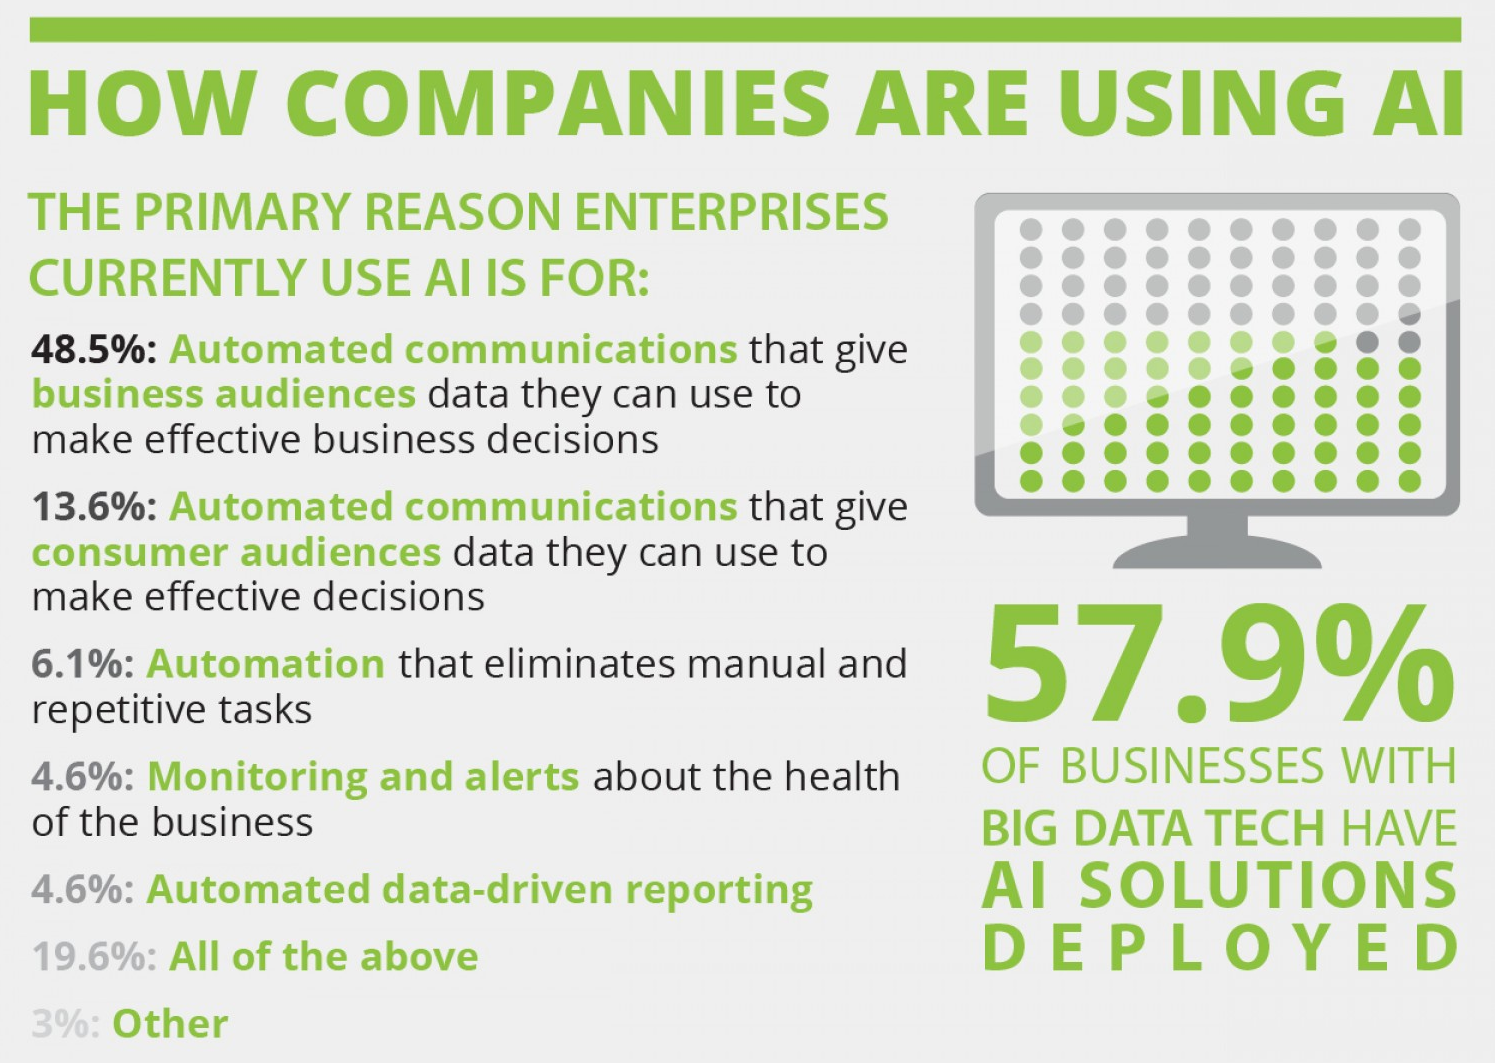
\includegraphics[width=0.85\textwidth,height=\textheight, keepaspectratio]{Figure3}
        \caption{Over 90\% of companies surveyed currently use some form of AI for automation.
                 \href{http://thumbnails-visually.netdna-ssl.com/artificial-intelligence-is-not-killing-jobs_557b4376e27b8_w1500.jpg}
                 {\textbf{Source}}}
      \end{figure}

    \paragraph{}
      Figure 3 highlights another statistic from the \textit{NarrativeScience}
      study referenced earlier. They found that over 90\% of respondents use AI
      primarily for automation. Many repetitive, mundane tasks can easily be
      done by intelligent machines. However, soon they will be able to take over
      more complex tasks as well.

    \paragraph{}
      Journalists Martin Dewhurst and Paul Willmott of McKinsey \& Company
      speculated that human workers ``...will be able to make the biggest difference
      through the human touch.''$_{[4]}$ In other words, humans will be needed to
      analyze the findings of intelligent machines and make critical
      decisions, like deciding the direction for the future of the company.

    \paragraph{}
      There is also a basic need in industry for “soft skills”, which Dewhurst and Willmott
      believe robots will never attain. At least in the foreseeable future, it
      is difficult to imagine humans willingly taking orders from a robot.
      Similarly, it seems unlikely that a robot leader could inspire the same
      drive into workers as a human leader. Emotion will likely be one of the
      most difficult things for intelligent machines to capture. Even once they
      do, conveying it in a way that is received well by humans is a whole other
      battle. Ultimately, the integration of AI will likely be similar to many
      other technological advances; it will change the way we work, but won't
      replace us.

  \section{Moving Forward}
    \paragraph{}
      While it may seem that intelligent machines have the ability to
      replace us, a machine is as likely to replace the human worker as a printer
      is. On one hand, a printer takes the job of a scribe who would have written the
      documents that it now prints. On the other hand, it frees up humans to
      do more important work. This is what intelligent machines will one day
      do as well.

    \paragraph{}
      Business leaders need to prepare their companies to adapt to
      changing tides, understanding that the role of humanity in the workforce
      is changing. However, humans will always have skills that robots do not.
      Eighty percent of respondents to the \textit{NarrativeScience} study believe
      that ``AI improves worker performance and creates jobs.''$_{[2]}$ If
      executives determine how to integrate AI and human workers in their company,
      there will be a twofold effect. First, it will keep
      most people employed, making money, and contributing to the economy.
      Second, it will make our companies more productive, further promoting a healthy
      economy.

  \cleardoublepage

  \restoregeometry

  \section{Citations}
    \begin{enumerate}[ {[}1{]} ]
      \item James Manyika, Michael Chui, Jacques Bughin, Richard Dobbs,
            Peter Bisson, and Alex Marrs (May 2013). ``Disruptive technologies:
            Advances that will transform life, business, and the global economy''
            \textit{McKinsey\&Company}.
            \href{http://www.mckinsey.com/insights/business_technology/disruptive_technologies}{\textbf{Link}}
            Last Accessed 2/11/16 \\
            \textit{Note: Some of the statistics I use are from the full report. There is a PDF download
                    link to it on the webpage linked above.}

      \item NA (2015). ``2015 State of Artificial Intelligence \& Big Data in
            the Enterprise'' \textit{NarrativeScience}.
            \href{https://www.narrativescience.com/filebin/images/Landing_Page/2015_State_of_AI_and_Big_Data_in_the_Enterprise.pdf}
                  {\textbf{Link}} Last Accessed 2/11/16

      \item Heath, Nick (ND). ``Why AI could destroy more jobs than it creates,
            and how to save them'' \textit{TechRepublic}.
            \href{http://www.techrepublic.com/article/ai-is-destroying-more-jobs-than-it-creates-what-it-means-and-how-we-can-stop-it/}
                 {\textbf{Link}} Last Accessed 2/11/16

      \item Martin Dewhurst, Paul Willmott (September 2014). ``Manager and
            machine: The new leadership equation'' \textit{McKinsey\&Company}.
            \href{http://www.mckinsey.com/insights/leading_in_the_21st_century/manager_and_machine}
                 {\textbf{Link}} Last Accessed 2/11/16


    \end{enumerate}

  \end{document}
